\documentclass{article}

\usepackage[utf8]{inputenc}
\usepackage[T1]{fontenc}
\usepackage[brazil]{babel}
\usepackage{sbc-template}
\usepackage{graphicx}
\usepackage{listings}

\renewcommand*\lstlistingname{Algoritmo}

\title{Protótipo de \emph{Interface} Humano Computador para Supermercados
Utilizando Técnicas de Lojas Virtuais e Computação Ubíqua}
\author{Wanderson Henrique Camargo Rosa\inst{1} \and Roberto Raguze
Flores\inst{1}}
\address{Centro de Ciências Exatas e Tecnológicas\\Universidade do Vale do Rio
dos Sinos (UNISINOS)\email{\{wandersonwhcr \and roberto.raguze\}@gmail.com}}

\begin{document}

\maketitle{}

\begin{abstract}
The electronic commerce is a virtualization of the traditional market stores
with the addition of search mechanisms made possible by computer tools. However,
the physical contact with the desired objects make people fear online marketing.
Therefore forcing people to move to the closest store and not being able to use
the features of the internet. This document presents ideas to apply interesting
elements from the virtual and real worlds in a traditional physical supermarket,
with the addition of augmented reality features through mobile devices.
\end{abstract}

\begin{resumo}
O comércio eletrônico é uma virtualização das lojas tradicionais, com adicionais
de facilidade de pesquisa, utilizando ferramentas computacionais. Porém, o
contato físico com os objetos de desejo faz com que muitas pessoas tenham receio
em compras \emph{online}, deslocando-se para o estabelecimento mais próximo e
não desfrutando destas ferramentas. Idéias para aplicação das ferramentas
interessantes do mundo virtual e real são aplicadas em um supermercado neste
documento, adicionando características de realidade aumentada através de
dispositivos móveis.
\end{resumo}

\section{Introdução}
\label{sec:introducao}

% Contextualização Geral

A utilização de ambientes virtuais para compras através de lojas eletrônicas
está cada vez mais comum nos dias de hoje. Através deste método de venda é
possível atingir mais facilmente o público alvo com promoções, dicas de produtos
semelhantes e comparação de preços.

% Negativos de Lojas Virtuais

Porém estes ambientes não fornecem ao cliente a principal característica de
venda de um produto: o contato direto. O ato do contato físico com produto pode
ser a ação chave para a compra do mesmo ou escolha de outros itens semelhantes,
algo que somente um comércio tradicional pode nos fornecer.

Se por um lado a informatização nos traz a facilidade de comunicar as pessoas
sobre o produto em questão, a venda tradicional pode nos dar uma melhor
segurança durante a compra. Porém, durante a compra comum, clientes enfrentam a
falta de informações de um determinado produto, recorrendo à pesquisa de dados
adicionais em lojas virtuais \cite{vonreischach2009}.

% União das Idéias

Dado que ambos os lados possuem características interessantes, podemos
desenvolver uma \emph{interface} para uma loja comum, trazendo as facilidades
virtuais para o mundo real, através de ambientes de realidade aumentada.

% Seções

A Seção \ref{sec:ihc} trabalha com a idéia sobre como será modelado o ambiente e
quais são as ferramentas que serão utilizadas e escolhido o ambiente a ser
aplicado. O sistema aplicado ao ambiente de supermercado escolhido será tratado
na Seção \ref{sec:sistema}. A prototipação do sistema, com descrições de telas e
algoritmos em formato GOMS são exibidos na Seção \ref{sec:prototipacao}. Por
fim, conclusões sobre o trabalho e o futuro de aplicações semelhantes são
debatidas na Seção \ref{sec:conclusao}.

\section{Interação Humano Computador}
\label{sec:ihc}

% Realidade

Em um estabelecimento real, um produto fica disponível ao consumidor, podendo
este interagir com o objeto. Informações adicionais podem ser fornecidas por
funcionários da loja, contudo, nem sempre a pessoa responsável pela venda
conhece completamente todos os produtos da loja ou pode fornecer dados técnicos
especializados, muito menos sugestões de todos os clientes que já compraram o
objeto.

% Realidade Aumentada

Por meio de dispositivos móveis, o cliente poderá acessar informações
pertinentes a qualquer produto da loja, pesquisar sobre produtos disponíveis e
em promoção, bem como controlar sua compra atual.

As informações serão acessadas em tempo real e os dados do cliente podem ser
salvos, visando criar ambientes do sistema especializados para cada pessoa,
estudando os produtos já comprados por ela e sugerindo novos. Com o cadastro
também é possível que o cliente efetue um pagamento \emph{online} dos objetos,
evitando filas em caixas de pagamento.

\subsection{Acesso aos Dados}

% Como é a Captura

O cliente, ao entrar na loja, terá duas opções de acesso ao sistema: utilizando
um leitor óptico fornecido ou instalando um aplicativo em seu próprio celular,
desde que este possua requisitos como acesso \emph{wi-fi}, câmera digital e
navegador \emph{web}. Estas são as características dos celulares atuais,
chamados \emph{smartphones}.

% Sistema Deverá Fazer

O sistema estará disponível utilizando uma rede sem fios interna ao recinto. Ele
deve armazenar dados sobre todos os produtos disponíveis na loja e controlar as
compras dos clientes. Portanto, cada pessoa que está em compras no
estabelecimento deverá efetuar autenticação no sistema, utilizando o dispositivo
móvel.

% Utilização de QRCode

Para acesso facilitado às informações do produto no dispositivo, cada objeto
deverá receber um código de barra de duas dimensões \cite{alapetite2010}. Estes
códigos contém um endereço no sistema interno para acesso à descrição, onde o
cliente poderá inclusive selecionar a quantidade desejável de objetos e
adicioná-los ao carrinho de compras virtual e real \cite{dix2000}, conforme seja
necessário.

% Ações Possíveis

Utilizando esta característica, o cliente poderá acessar informações mais
detalhadas do produto, como dados técnicos ou valores energéticos, comparar
preços e melhores dias para compras, bem como fornecer sugestões do produto para
terceiros \cite{canny2006} ou acessar futuras promoções da loja.

% Conclusão do Acesso aos Dados

Assim, o rápido acesso às informações de produto poderão ser incluídas em
ambientes reais, trazendo os meios virtuais para a realidade, extendendo-a. O
usuário terá todos os dados disponíveis do produto que está comprando e poderá
vê-lo, unindo o melhor dos dois ambientes.

\subsection{Idealização}

% Aplicação Focada

Com esta análise de informações, há uma proposta de criação de uma
\emph{interface} para supermercados que utilize técnicas de lojas virtuais,
tornando a compra mais fácil e controlada, através de dispositivos móveis.

% Público Alvo

Temos então como público alvo todas as pessoas que utilizam o ambiente do
supermercado e que já estão acostumadas aos padrões comuns. O sistema deve ser
capaz de facilitar as compras, dando comodidade e segurança ao cliente.

% Necessidades

Não podemos esquecer que nem todas as pessoas estão acostumadas com tecnologias
diferenciadas. Portanto, quanto mais a \emph{interface} estiver adaptável ao
usuário, melhor será o retorno e satisfação do cliente.

\section{Sistema e Ambiente}
\label{sec:sistema}

% Necessidades Básicas

O sistema é acessível através de uma rede sem fio disponível e pode ser
visualizado em dispositivos móveis previamente descritos. Qualquer usuário deve
estar apto para utilização. Buscando rapidez de aprendizado, o sistema possui
algumas caracteristicas descritas abaixo.

\subsection{Inicialização do Sistema}

% Tutorial

Para treinar o usuário sobre a utilização do sistema, ele poderá ser convidado a
selecionar algum produto em uma lista de compras comuns. Um passo-a-passo poderá
ser feito através do sistema, seguindo cada instrução no estilo \emph{tutorial}.

\subsection{Dicas para Usuário}

% Tooltips para Usuários

O sistema pode capturar uma sequência de entradas frequentes do usuário e
fornecer dicas de como estas tarefas podem ser otimizadas, através de teclas de
atalhos ou botões que podem ser adicionados à tela inicial do sistema.

Também deve ser fornecido em locais estratégicos (lancherias internas,
atendimento ao consumidos, videos em exibição contínua sobre a utilização do
sistema.

\subsection{Localização}

% Localização e Dicas Conforme Corredor

Ao movimentar-se dentro do supermercado, o cliente pode ser informado sobre
promoções ou produtos em destaque no corredor atual. Isto pode ser adicionado
aos dispositivos que possuem posicionamento GPS e conforme efetue seu
deslocamento, ele não é informado por produtos que procura, mas sim com dicas de
elementos e promoções inexperadas \cite{canny2006}.

\subsection{Pesquisa}

% Pesquisa de Produtos

Um produto pode ser pesquisado pelas suas características no sistema. Além de
fornecer dados do produto como descrição, especificações opiniões sobre o
produto e sugestões, ele também é capaz de exibir os locais onde os produtos
podem ser retirados, através de mapas e localização GPS.

% Favoritos e Histórico

Produtos podem ser gerenciados através de favoritos, para rápido acesso e
comparação de preços. Também é necessário manter um histórico das pesquisas,
pois a reentrada dos dados pode ser uma tarefa dificultada, tendo em vista que
dispositivos móveis nem sempre possuem teclados completos.

\subsection{Controle de Produtos}

% Produtos no Carrinho

O usuário poderá visualizar e gerenciar os produtos do carrinho através do
sistema. Também poderá ser incluído um valor máximo especulado pelo usuário para
controle de gastos. Assim, o cliente terá controle total e pode visualizar o
preço de cada produto que será pago a qualquer momento.

\section{Prototipação}
\label{sec:prototipacao}

% Tela Principal do Sistema

A tela principal do sistema busca centralizar as ações mais utilizadas pelos
usuários, descrita na Figura \ref{fig:main}. Os botões centrais indicam ações de
pesquisa, lista de compras, produtos favoritos, carrinho de compras atual,
histórico de compras e pesquisa e seção de atendimento ao consumidor. Abaixo,
temos a exibição das promoções, que podem ser visualizadas com deslizamento
horizontal.

\begin{figure}[ht]
    \centering{}
    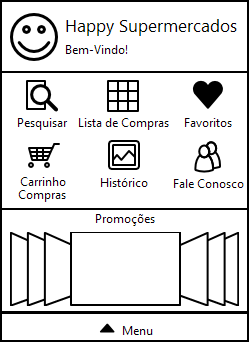
\includegraphics[scale=0.4]{images/main.png}
    \caption{Tela Principal do Sistema}
    \label{fig:main}
\end{figure}

% Tela Principal de Produto

A tela após a captura do código de barras do produto pode ser exemplificada
conforme Figura \ref{fig:produto}. Podemos verificar que o nome do produto atual
está na parte superior em maior tamanho de fonte, para primeira verificação se a
captura foi concluída com sucesso.

\begin{figure}[ht]
    \centering{}
    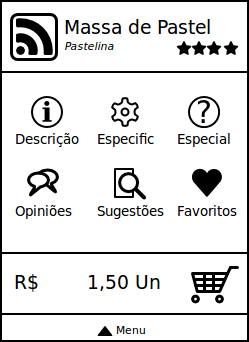
\includegraphics[scale=0.4]{images/produto.png}
    \caption{Descrição do Produto}
    \label{fig:produto}
\end{figure}

Cada ação disponível para o produto está visível na área central, exibidos com
ícones que fornecem uma identificação rápida conforme método que executam,
característica de engenharia semiótica.

O preço do produto também é visível de forma destacável. Para mais opções, há um
atalho ao menu principal do sistema na base, com uma flecha apontando para cima,
indicando que ele será deslizante.

% Tela do Carrinho de Compras

O carrinho de compras virtual trabalha como descrito na Figura \ref{fig:compra}.
As imagens representantes dos produtos são visualizadas conforme
\emph{interfaces} dos produtos atuais, que respeitam uma perspectiva de livros
em uma estante.

\begin{figure}[ht]
    \centering{}
    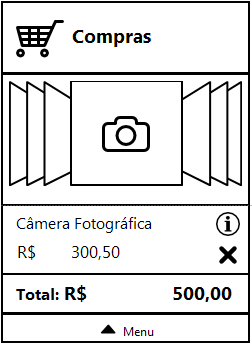
\includegraphics[scale=0.55]{images/compra.png}
    \caption{Carrinho de Compras}
    \label{fig:compra}
\end{figure}

O produto pode ser acessado no botão de informações e poderá ser excluído no
botão de remoção, que utilizam como característica de outros sistemas o mesmo
formato de ícones representantes. A visualização da quantia total em gastos é
visível de forma destacável. A finalização da compra é interna ao menu
deslizante, evitando com que o usuário efetue esta ação acidentalmente.

\subsection{GOMS}

Para utilização de GOMS, devemos definir os usuários do sistema, conforme
Algoritmo \ref{goms:usuario}. A pesquisa de produtos no sistema pode seguir a
lógica descrita pelo Algoritmo \ref{goms:pesquisa}. O usuário possui três
elementos para busca: nome do produto, marca ou categoria. A compra de um
usuário é descrita no Algoritmo \ref{goms:compra}. Por fim, para ação de
cadastro de cliente, pode-se seguir o Algoritmo \ref{goms:cadastro}.

\begin{footnotesize}
    \lstinputlisting[basicstyle=\ttfamily,caption={Usuario},label=goms:usuario,captionpos=b]{resources/usuario.goms}
\end{footnotesize}

\begin{footnotesize}
    \lstinputlisting[basicstyle=\ttfamily,caption={Pesquisa},label=goms:pesquisa,captionpos=b]{resources/pesquisa.goms}
\end{footnotesize}

\begin{footnotesize}
    \lstinputlisting[basicstyle=\ttfamily,caption={Compra},label=goms:compra,captionpos=b]{resources/compra.goms}
\end{footnotesize}

\begin{footnotesize}
    \lstinputlisting[basicstyle=\ttfamily,caption={Cadastro},label=goms:cadastro,captionpos=b]{resources/cadastro.goms}
\end{footnotesize}

\section{Conclusão}
\label{sec:conclusao}

A idéia de trazer a realidade aumentada para objetos comuns não é novidade.
Dispositivos móveis como celulares, possuem hoje o mesmo processamento de
computadores pessoais de doze anos atrás \cite{canny2006}, porém seu poderio é
gasto com desempenho para mídias.

Se utilizarmos todas as ferramentas disponíveis nestes aparelhos, como sistemas
de posicionamento global, acelerômetro e giroscópio, podemos criar ferramentas
de manipulação de objetos virtuais em um campo tridimensional.

O estudo destas aplicações não eram estudadas antigamente pois não eram
necessárias no contexto de utilização de computadores. Um programa para
reconhecimento de voz não é necessário em um escritório, onde existe métodos
mais simples de entrada de informações.

Porém, ambientes onde dispositivos possuem métodos minimizados de entrada e com
facilidade em reconhecimento de voz, como celulares, podem usufruir desta
tecnologia, popularizando estas técnicas.

Conforme o público alvo, estas tecnologias devem ser desenvolvidas com cuidado,
pois cada grupo possui características distintas. Se, um aplicativo consegue ter
adaptação para cada grupo alvo, podemos ter uma grande abrangência e aceitação.

Trazer usuários virtuais para o uma loja comum pode ser uma estratégia, pois os
elementos interessantes de cada mundo é aplicado utilizando a técnica descrita
neste documento.

\bibliographystyle{sbc}
\bibliography{sbc-template}

\end{document}